% !TEX encoding = MacOSRoman

\documentclass[a4paper,12pt]{article}

\usepackage{listings}
\usepackage[parfill]{parskip}
\usepackage{float}
\usepackage{graphicx}
\usepackage[swedish]{babel}
\usepackage[applemac]{inputenc}
\usepackage[margin=35mm]{geometry}
\usepackage{fancyhdr}
\usepackage[encapsulated]{CJK}
\usepackage{inconsolata}
\usepackage{amssymb,amsmath}


\newenvironment{ppl}{\fontfamily{ppl}\selectfont}{}
\newenvironment{inconsolata}{\texttt}{}


\DeclareGraphicsRule{.tif}{png}{.png}{`convert #1 `dirname #1`/`basename #1 .tif`.png}

\begin{document}

\begin{titlepage}
\begin{center}


\textsc{\Large Link�ping University}

\rule{\linewidth}{0.5mm} \\[2cm]

\textsc{\Large Charactarezation of multilayer ScCr on Si}\\[10cm]

\normalsize Mattias Jansson - matja307@student.liu.se\\[0.5 mm]
Simon Larsson - simla804@student.liu.se\\[0.5 mm]
Link�pings universitet\\[0.5 mm]
Link�ping\\[0.5 mm]
2014-03-26\\

\end{center}
\end{titlepage}

\newpage

\section{Abstract}
\emph{Express subject of the results}


\section{Introduction}
\emph{Includes: General background, Literature review, gap sentence, statement of purpose}

\section{Experimental Details}
\emph{What did I do? (Must include sufficient detail so that the results can be duplicated.}

A sample prepared for transmission electron microscopy was examined using TEM. The TEM used a LaB6 filament electron gun with an acceleration voltage of 200 kV. Both micrographs of the real space structure and diffraction measurements were taken. 

The sample was examined using X-ray diffractometry (XRD). The measurements were done using a copper filament X-ray source. The method used was low angle x-ray reflecivity. The angle $\theta$ is defined as shown in figure \ref{fig:xrd3}.

\begin{figure}[h]
\begin{center}
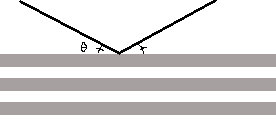
\includegraphics[scale=0.6]{xrd_plot3.png}
\caption{Defenition of angle $\theta$ for XRD measurements
\label{fig:xrd3}}
\end{center}
\end{figure} 


\section{Results}
\emph{What did I get? What did I observe?}


\begin{figure}[h]
\begin{center}
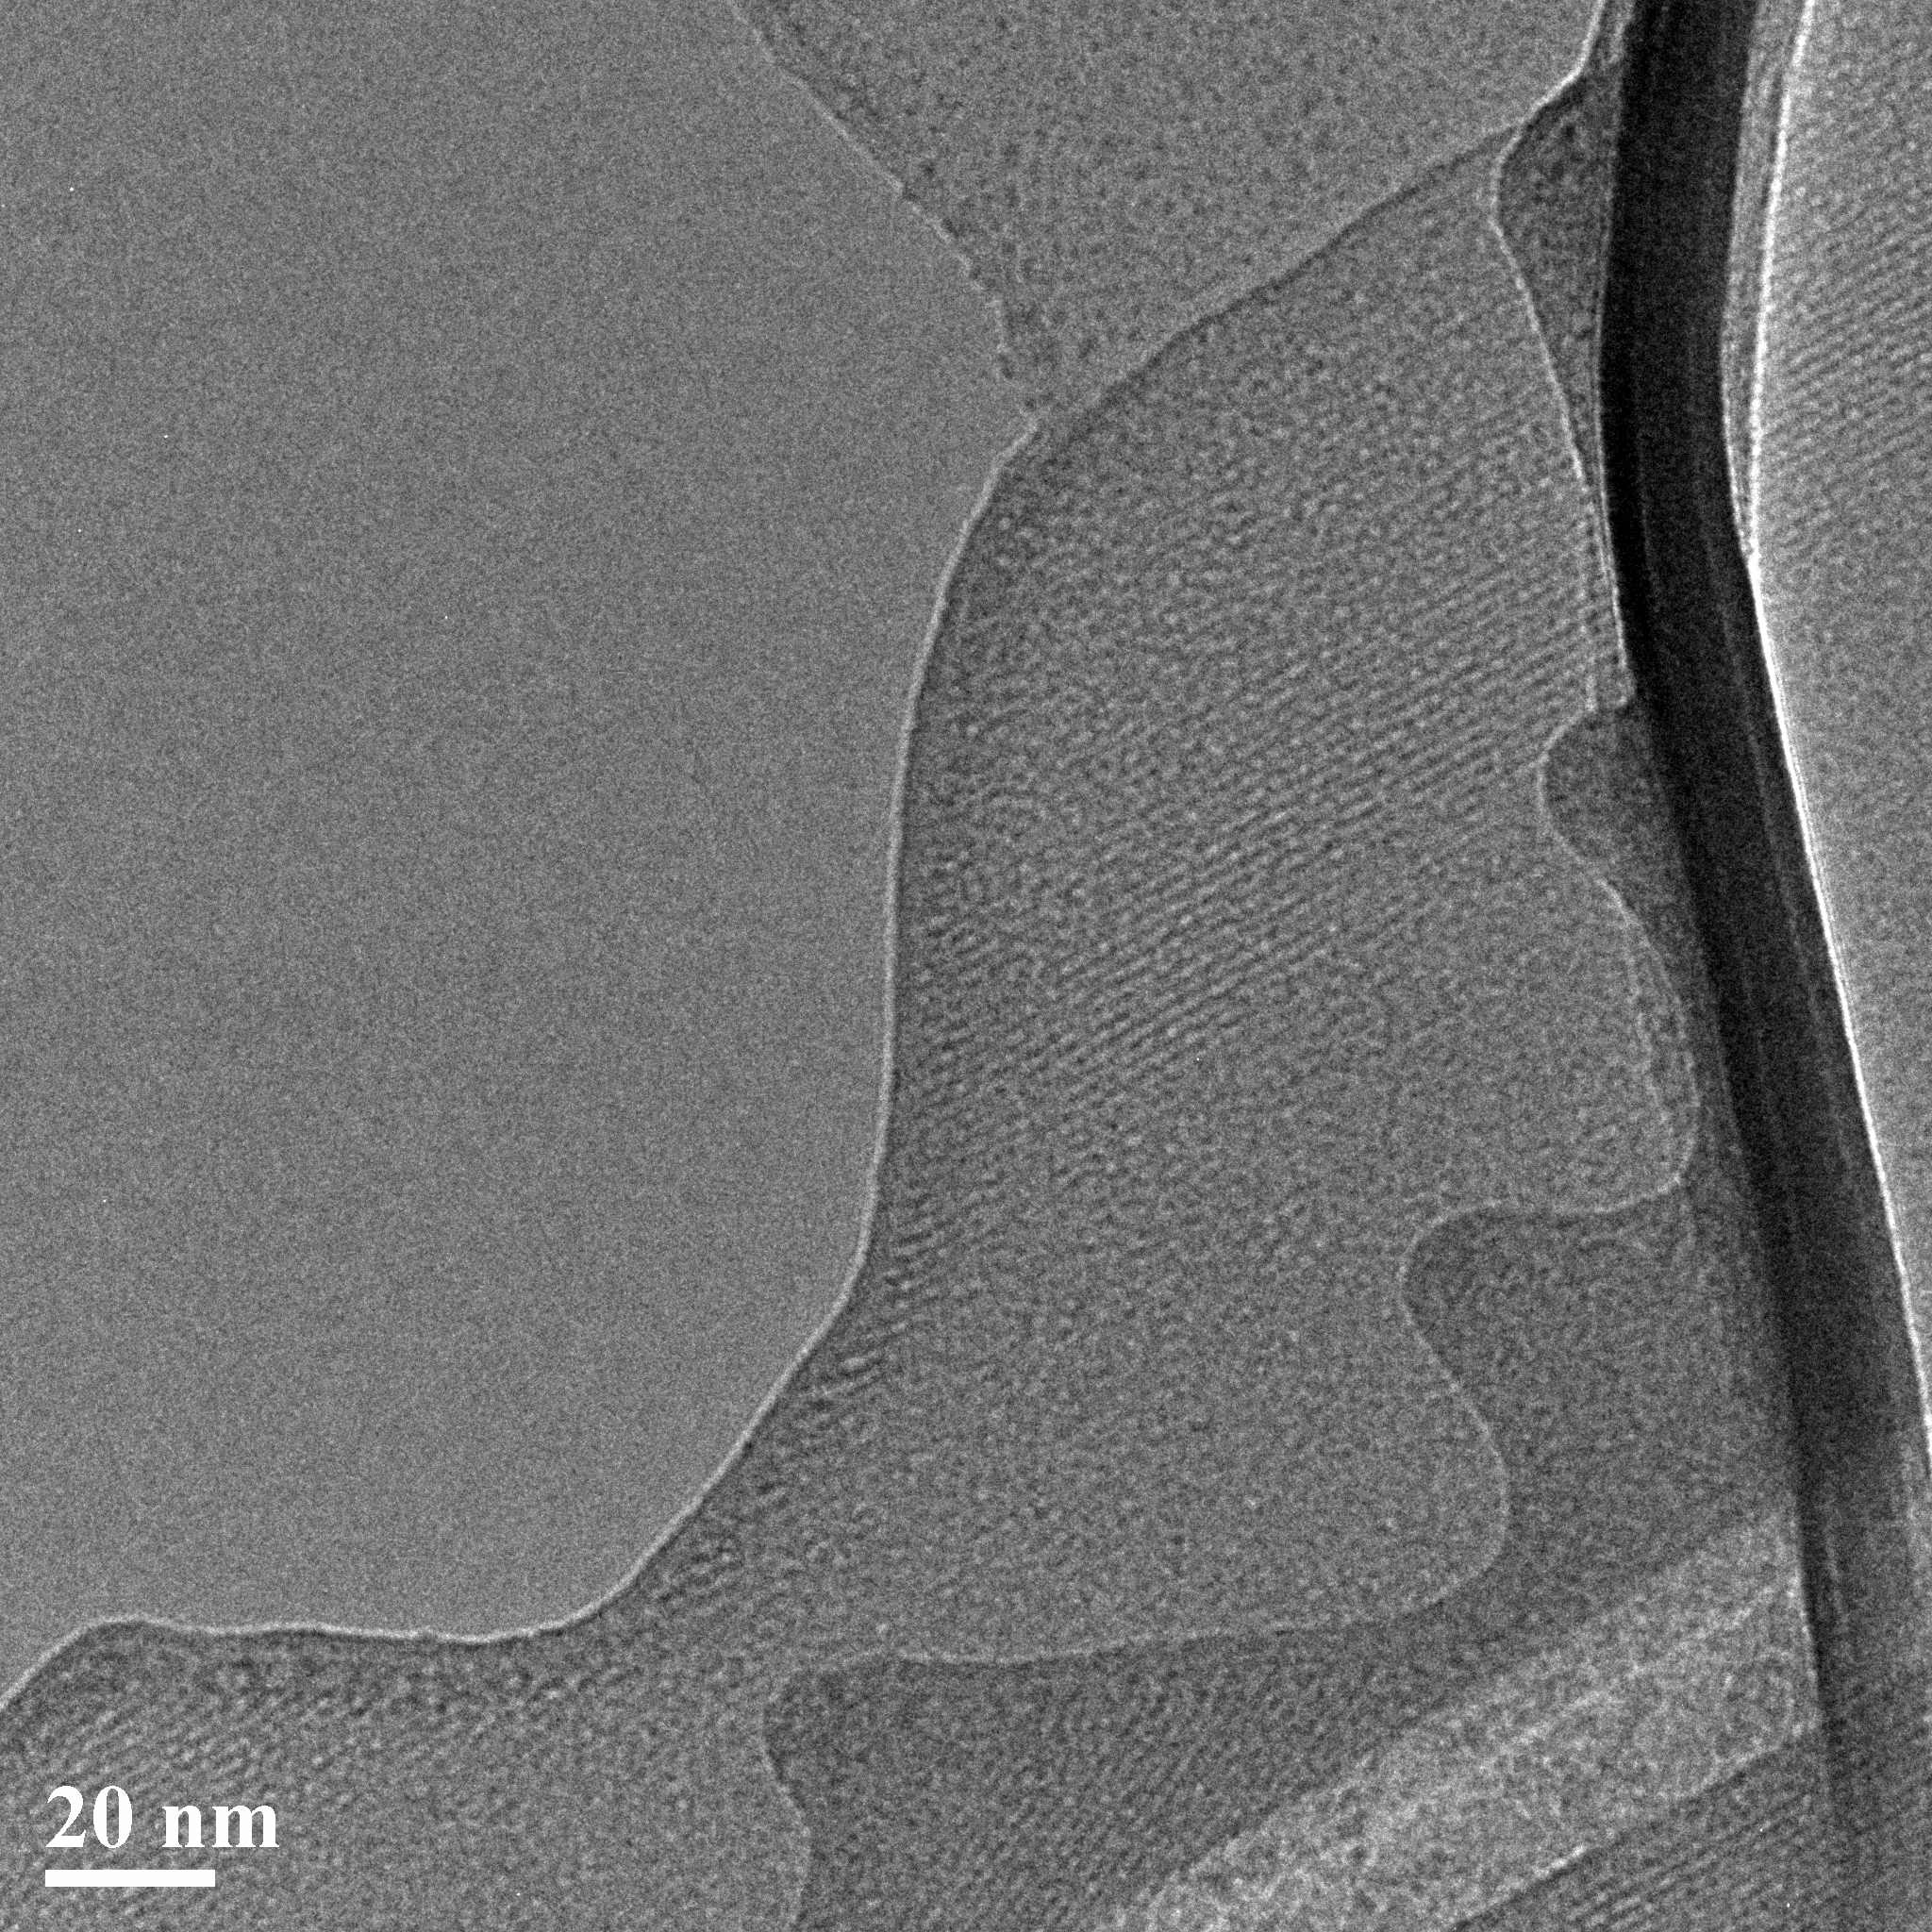
\includegraphics[scale=0.15]{tem1.png}
\caption{Low magnification image of layer structure
\label{fig:tem1}}
\end{center}
\end{figure}


\begin{figure}[h]
\begin{center}
\includegraphics[scale=0.15]{tem2-2.png}
\caption{High magnification TEM image with size measurement of ten layers. 
\label{fig:tem2}}
\end{center}
\end{figure}

Figure \ref{fig:tem1} shows an overview image of a part of the CrSc layer structure. Figure \ref{fig:tem2} shows a higher magnification image. The line in figure is a direct measurement of the size of ten layers, thus one layer is found to be:

\[D \approx 1,64 nm\]

Figure \ref{fig:xrd1} shows the XRD spectrum from the low angle x-ray reflexivity measurements. The figure clearly shows two peaks at $2\theta = 5$ and $2\theta = 10$ respectively. 

\begin{figure}[h]
\begin{center}
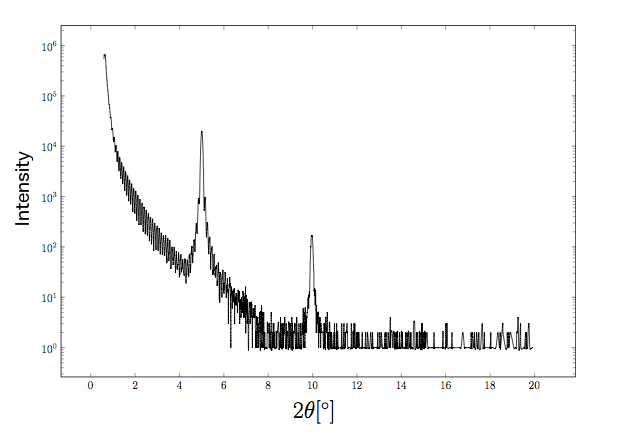
\includegraphics[scale=0.6]{xrd_plot1.png}
\caption{Low angle XRD measurement. 
\label{fig:xrd1}}
\end{center}
\end{figure}

The peaks correspond to two solutions to Bragg's law for thin layers:

\begin{equation}
\label{eqn:bragg}
m\lambda = 2D\sin\theta\sqrt{1+\frac{\eta^2-1}{\sin^2\theta}}
\end{equation}

Figure \ref{fig:xrd2} shows a measurement of the lower $\theta$ part of the spectrum. This shows that there are no bragg peaks in this part of the spectrum. Hence the $\theta = 5$ peak is the $m = 1$ peak. 

\begin{figure}[h]
\begin{center}
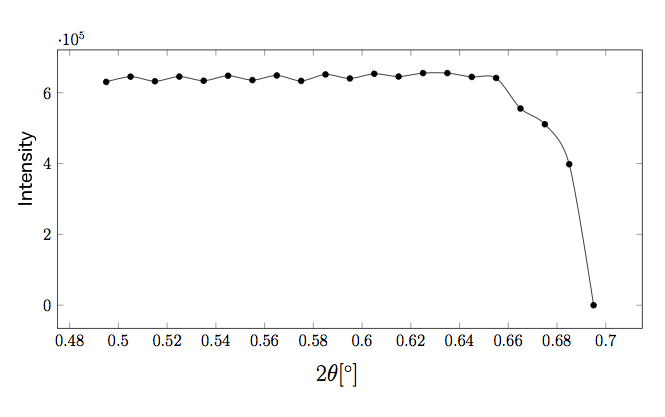
\includegraphics[scale=0.6]{xrd_plot2.png}
\caption{Low $\theta$ part of spectrum for low angle XRD measurement. 
\label{fig:xrd2}}
\end{center}
\end{figure}

To find the layer period thickness, $D$, (\ref{eqn:bragg}) is rewritten as: 

\begin{equation}
m^2 = \frac{4D^2}{\lambda^2}\sin^2\theta + C
\end{equation}


Where C is a constant w.r.t. $\theta$. Using the two peaks for m = 1 and 2 respectively, we get figure XXX3, giving:

\[\frac{4D^2}{\lambda^2} \approx 532.07 \]

or
\[ D \approx 17.8 \AA. \]
\section{Discussion}
\emph{So what? Interpret the results.}

\section{Conclusion}
\emph{Think of three things that the reader should remember.}

\end{document}








































